%!TEX root = ../main.tex
\chapter{Design}
In this section, I will discuss both aesthetic and technical designs for the application as well as offer an overall design of the system as a whole.

\section{User Interface}
\subsection{Navigation}
A focus must be put on the usability of the screens in KidQuest.
They should not only be easy to use, but easy to learn and navigate between, and should offer minimal resistance in the use of the application.

\cite{stone2005user} classifies a good user interface design as an `easy, natural and engaging interaction between a user and a system'.

\subsection{Android Developer Guidelines}

\subsection{Wireframes}
Wireframing is a useful tool to plan out the aesthetic design of screens and the UI elements used within them. 
A wireframe is also useful to get a better overview of the navigation between screens, as they can be used to plan out the button presses that will select the next screen.
The wireframes shown in appendix \ref{appendix:wireframes}


\section{System Design}
\begin{figure}[ht]
	\centering
	\includegraphics[scale=0.55]{images/SystemDiagram.png}
	\caption{System Design Diagram}
	\label{fig:systemdesign}
\end{figure} 


\section{User Requirements}
\subsection{The Child}
The child will open the application and be met with a character screen, which will display the relevant information about their character, including the XP/Gold they currently have, the XP needed until the next level and the recent rewards they have earned.
The child can then check their quests and mark any that they have finished as complete.
The quest will then move into the pending quest log, ready for a parent to confirm.
Once the parent has confirmed the quest, the child will be met with a reward of experience points and gold based on the difficulty of the quest.

The child can visit the rewards section to spend their gold on in-game items which will increase the power level of their character. 
Alternatively, they can spend their gold on rewards that have been set by the parents. 
i.e. 400 gold will be able to purchase a visit to the cinema.

As an incentive to collect the rewards offered in-game, the child will be able to add friends in the game and challenge them to in-game battles. 
The result of the battle will be generated via the current level and equipment that the character has equipped. 
For the purposes of safety, friend requests must be confirmed by the parent before the friend request is confirmed.

The application controls must be kept simple and uniform so that they are able to be learned and used by children.
Children will not be able to access any parent functions as they will require the parent's pin code. 

\subsection{The Parent}
The parent can either access the parent functions on the child's application using a pin code, or use their own `parent edition' of the application. 
When designing the use case of the parents, it is important to minimize the level of interaction required from the parent to ensure they do not become tired of managing the game for the child.

The parent can create quests through a simple interface, entering in the task's name, an optional description and a difficulty level. 
The quest can have one of 5 difficulty levels, ranging from very hard to very easy.
The game will generate the rewards for the child based on their current level and the difficulty of the quest.
Alternatively, the parent can choose from a range of preset quests from three selected categories:
\begin{itemize}
	\item 
		Staff Pick - A list of common tasks chosen by the me to help populate the list with easily selectable quests. 
		This will contain obvious choices for tasks such as ``Clean your room'' or ``Wash the dishes''
	\item
		Trending in Your Area - A list of tasks that have been recently trending in the users location. 
		This will be used to suggest tasks that many users have been inputting into the app, including recently relevant tasks like ``Rake the leaves in the garden'' at the start of Autumn.
	\item 
		Trending Amongst Friends - Tasks that have been trending amongst the users friends list, not including quests counted in the previous 	trending category. 
		This may include friends added both within the app and/or friends from Facebook integration.  
\end{itemize}

\section{Development Methodologies}
\subsection{Agile}
As I am a single developer working on this project, this is beneficial to me as it helps give early sight of potential design issues early in the project.

\section{Development Processes}
There are also many sub-processes that are born out of or tie into Agile which could be beneficial for my project.

\subsection{Test-Driven Development}
From the various development processes I have examined, I have chosen to use test-driven development as my key driving force 

However, it must also be considered that if the practice offers a higher quality of code it is inherently likely to produce less errors and therefore the productivity/time trade-off may be worth it.
It is also noted that I must be prepared as I am unfamiliar with TDD myself, and will likely experience a similar drop in productivity as I begin to practice the methodology, however the paper offered several useful tips for developers/teams who are new to the practice.

\subsection{Behaviour-Driven Development}
After planning out the requirements, the next step in the design of KidQuest was to plan out the database structure.
I created an entity relationship to map out the various tables needed and the relationships between them.

\begin{figure}[t]
	\centering
	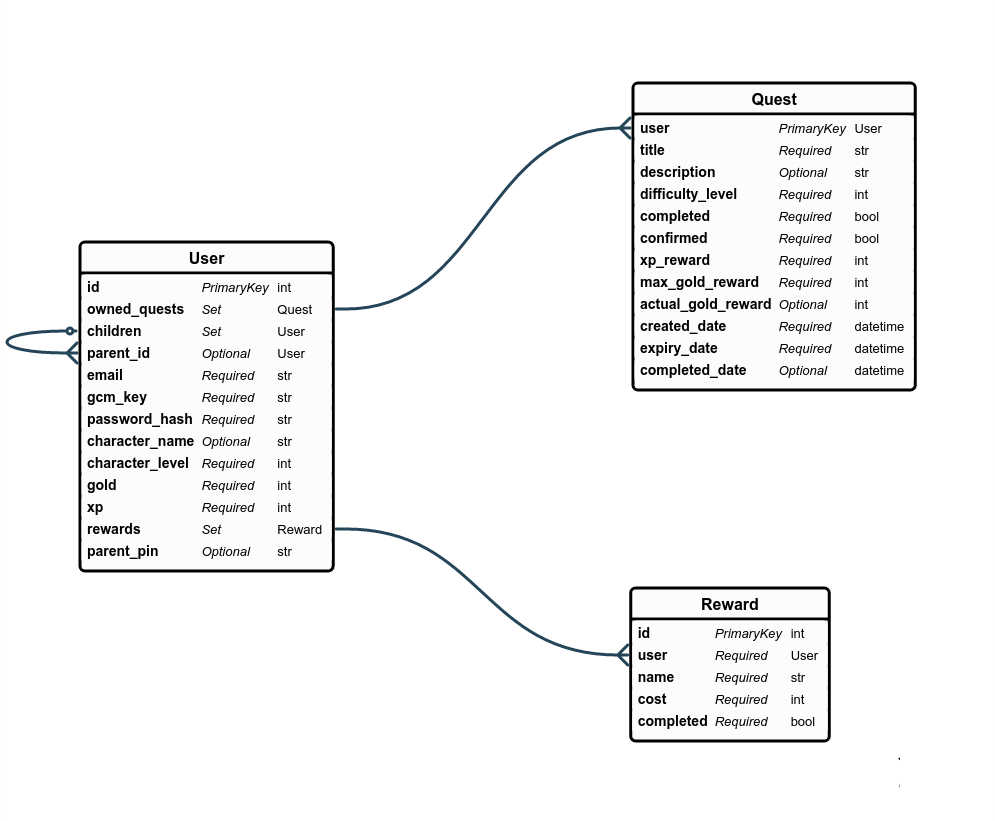
\includegraphics[width=0.75\textwidth]{images/entityRelationshipDiagram.png}
	\caption{Entity-Relationship Diagram}
	\label{fig:ERD}
\end{figure}

I have chosen to create the application in the Android SDK largely due to my previous experience with Java and Android. 
Furthermore, I believe Android is more applicable to the target audience of the app, as Android owns 82.8\% of the smartphone market share as of 2015.
%http://www.idc.com/prodserv/smartphone-os-market-share.jsp
I believe that parents are also more likely to buy their children Android phones than other brands due to the lower price point, making them more appealing when considering the likelihood of them being lost or broken by a child.

For the data analytics, I have opted to use web services written in Flask microframework for python, hosted on a server running Ubuntu Server 14.04. 
I have chosen python due to it's strong backing and community support in data analytics, and is one of the main languages of choice for scientists and statisticians.
The flask framework was chosen specifically as it is very simple to write and host RESTful APIs over the web.

To safely store and version control the code, I used a GitHub private repository to host my code in cloud storage. 
This allows me to better manage changes to the code-base. 

\section{Development Style}

\section{Testing}
Unfortunately, when developing a REST API, it is difficult to manually write and send the request to the API to test it.
Programs and scripts exist to ease the process somewhat, but I found the easiest way to be automating the requests entirely. 
As a main principle of REST is to plan out the specific endpoints that can be messaged, it becomes rather simple to plan out tests in the form of sending an example of a valid and invalid request of each request type to each endpoint.
For example, the endpoint of `/api/users/<userId>/' allows two request types, GET and PUT, which generates four test cases.
\begin{itemize}
	\item{Valid GET}
	\item{Invalid GET}
	\item{Valid PUT}
	\item{Invalid put}
\end{itemize}  
%TODO: Research what test generation this is
However, this raises issues when considering that a request could be invalid for multiple reasons, and simply testing for invalid/valid may not reach adequate code coverage.
An example of this could be that a PUT request may be invalid due to an email address already existing within the database or because they have not included a valid did not include any new data about the user, which are two separate sections of the code that arguably each require their own tests.
Because of this, it must be analysed whether or not the test cases achieve sufficient code coverage, rather than just relying on the entry points into the software.
Luckily, the python package `coverage.py' allows for simple analysis of unit tests to determine the current code coverage for tests, which will provide a higher rate of confidence.

\subsection{Unit Testing} 
Unit Testing is integral to the workflow of test-driven development

\subsection{Integration Testing}
Integration testing encompasses tests that specifically test that the various parts of the project work together correctly.
For example, integration tests for KidQuest would test that the server and mobile app are able to correctly function together, by ensuring that the app can correctly send requests and that the server receives those requests as they were sent.


\subsection{Black Box Testing}

\subsection{White Box Testing}


\subsection{Regression Testing}
Regression testing is the practice of retesting the previously tested parts of the software to ensure that they are still performing correctly after a change elsewhere in the code, it can also be used to describe the process of testing previously detected and fixed bugs to determine that they have not reappeared.
This is made significantly easier by the implementation of strong automated unit tests, which allow me to quickly retest the majority of the code by rerunning the test suite.
I also intend to follow a common development practice where a unit test is added for each defect that is found within the code, a new unit test is added to detect the presence of that bug specifically. 
This will allow me to easily spot any recurrences of legacy bugs that would otherwise go unnoticed.

